\chapter{Ottimizzazione}
Una delle parti più importanti del Deep Learning è quella legata alla parte di \textbf{Ottimizzazione}. Fino ad ora, noi conosciamo lo 	\textbf{Stochastic Gradient Descent}, sappiamo però che molto spesso implementandolo attraverso le sue varianti (Batch, MiniBatch, ecc\dots), si possono incontrare diversi problemi nell'allenare il modello. Dunque, questo capitolo ha lo scopo di andare oltre queste metodologie tradizionali per ottimizzare il nostro modello. La superficie d'errore in cui ci ritroviamo può essere rappresentata da una parabola o, in più dimensioni, da una sfera. Tuttavia, nella pratica, le nostre curve di errore assumono la forma di ellissi, poiché le scale delle varie feature sono diverse fra loro (Figura~\ref{fig:error_surface}). Pertanto, la discesa del gradiente diventa inefficiente, subendo rallentamenti e oscillazioni, che ne compromettono la convergenza.

\begin{figure}[h]
\centering
\includegraphics[width=0.55\textwidth]{figure/error_surface.png}
\caption{Rappresentazione della superficie d'errore}
\label{fig:error_surface}
\end{figure}

\section{Discesa del Gradiente}
Se il dataset risulta essere altamente ridondante, il gradiente nella prima metà dei dati sarà praticamente identico a quello presente nella seconda metà. Dunque, invece di calcolare l'intero gradiente, possiamo computarlo solo su una porzione dei dati e riutilizzarlo sulla restante parte. L'idea successiva a questa considerazione, è quella di utilizzare piccoli batch dell'intero dataset in modo tale che essi siano rappresentativi delle classi in analisi. Questo porta all'uso della discesa del gradiente stocastica con mini-batch, una soluzione che migliora l'efficienza computazionale e la stabilità dell'addestramento.

\subsection{Scegliere il learning rate}
Per poter scegliere il learning rate, inizialmente decidiamo di impostarlo a un valore elevato, in modo tale da evitare di collassare su un minimo locale troppo presto. Successivamente, attraverso tecniche di decay, lo riduciamo progressivamente per aumentare la probabilità di convergere verso un minimo globale o comunque un minimo locale migliore rispetto a quelli precedenti. Tra le strategie più comuni per il decay del learning rate possiamo considerare le seguenti:
\begin{itemize}
\item\textbf{Step Decay}: il learning rate viene ridotto di un fattore fisso dopo un certo numero di epoche;
\item\textbf{Exponential Decay}: il learning rate diminuisce esponenzialmente nel tempo;
\item\textbf{Adaptive Learning Rate}: tecniche come Adam e RMSprop regolano dinamicamente il learning rate per ogni parametro della rete.
\end{itemize}

\begin{figure}[!ht]
    \centering
    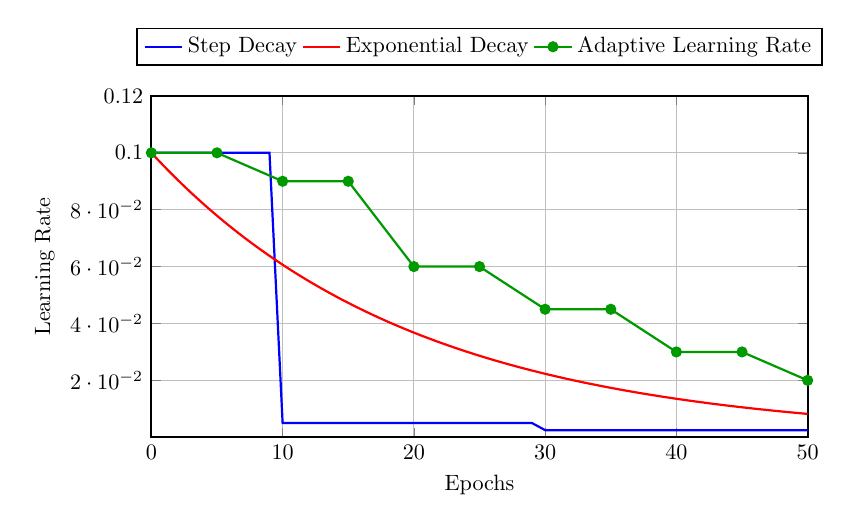
\begin{tikzpicture}[scale=0.8]
        \begin{axis}[
            width=12cm, height=7cm,
            xlabel={Epochs},
            ylabel={Learning Rate},
            xmin=0, xmax=50,
            ymin=0, ymax=0.12,
            legend style={
                at={(0.5,1.2)},
                anchor=north,
                legend columns=3
            },
            xtick={0,10,20,30,40,50},
            ytick={0.02,0.04,0.06,0.08,0.1,0.12},
            grid=both,
            thick,
            every axis plot/.append style={line width=1pt},
        ]

        % Step decay
        \addplot[blue, domain=0:50, samples=51] 
            {0.1 * (x<10 ? 1 : (x<30 ? 0.05 : 0.025))};
        \addlegendentry{Step Decay}

        % Exponential decay
        \addplot[red, domain=0:50, samples=200]
            {0.1 * exp(-0.05*x)};
        \addlegendentry{Exponential Decay}

        % Adaptive (manually simulated)
        \addplot[green!60!black, mark=*] 
            coordinates {
                (0, 0.1) (5, 0.1) (10, 0.09) (15, 0.09)
                (20, 0.06) (25, 0.06) (30, 0.045)
                (35, 0.045) (40, 0.03) (45, 0.03) (50, 0.02)
            };
        \addlegendentry{Adaptive Learning Rate}

        \end{axis}
    \end{tikzpicture}
    \caption{Confronto tra diverse strategie di decadimento del learning rate.}
    \label{fig:lr_decay}
\end{figure}

\subsection{Inizializzazione dei pesi}
Un altro problema rilevante riguarda l'inizializzazione dei pesi nelle reti neurali. A differenza della regressione lineare, in cui l'ottimizzazione è più diretta, nelle reti neurali l'algoritmo di backpropagation può essere compromesso se i pesi iniziali non sono scelti correttamente. Se due pesi all'interno di uno stesso layer hanno valori iniziali identici, l'errore propagato attraverso la rete genererà aggiornamenti identici per entrambi, portando dunque alla simmetria dei pesi, questo impedirà alla rete di apprendere in maniera efficiente. Inoltre, se i pesi sono inizializzati con valori troppo grandi o troppo piccoli, si possono verificare problemi di vanishing o exploding gradient o ancora il problema dell'overshoot in cui non si giunge a convergenza, ma vi è un'oscillazione continua dei valori.

\subsubsection{Fan-in e Fan-out}
\marginpar{\href{https://proceedings.mlr.press/v9/glorot10a/glorot10a.pdf}{"Understanding the difficulty of training deep feedforward neural networks" by Xavier Glorot et al. (2010)~\cite{glorot2010understanding}}}
Il Fan-In e il Fan-Out sono concetti legati alla distribuzione dei pesi negli strati di una rete neurale e vengono usati in tecniche di inizializzazione dei pesi come quella Xavier (Glorot).
\begin{itemize}
    \item \textbf{Fan-in}: il numero di neuroni che alimentano un dato neurone in un layer successivo;
    \item\textbf{Fan-out}: il numero di neuroni che un dato neurone alimenta nel layer successivo;
\end{itemize}

\begin{Esempio}
    Consideriamo un layer completamente connesso (fully connected, FC) con: 256 neuroni in ingresso, dunque il fan-in sarà 256, e con 512 neuroni in uscita, dunque il fan-out sarà 512.
\end{Esempio}


L'inizializzazione dei pesi deve tener conto di questi valori per evitare che le attivazioni diventino troppo grandi o troppo piccole. Tecniche come Xavier prendono in considerazione questi aspetti, utilizzando distribuzioni gaussiane o uniformi adeguate. Basti pensare che nel momento in cui inizializiamo i pesi in maniera casuale, se venissero scelti con una varianza troppo grande, i valori dell'attivazione esplodono strato dopo strato (exploding activations). Se la varianza è troppo piccola, i segnali si riducono progressivamente (vanishing activations), rendendo difficile l'apprendimento.

\subsection{Xavier Initialization}
L’idea chiave della \textbf{Xavier Initialization} è scegliere i pesi in modo tale che:
\begin{enumerate}
    \item La varianza dell'output di un neurone sia simile alla varianza del suo input (per evitare esplosioni o annullamenti del segnale);
    \item La varianza dei gradienti rimanga costante tra gli strati (per evitare la degenerazione del training);
\end{enumerate}
Consideriamo $x$ l'input di un neurone e $W$ il vettore dei suoi pesi, l'output del neurone pertanto sarà dato da $z=Wx$, se supponiamo che $x$ abbia media nulla e varianza $\operatorname{Var}[x]$, allora la varianza del nostro output sarà chiaramente $\operatorname{Var}[Wx]$. Se assumiamo che i pesi e gli input siano indipendenti fra loro e che i pesi abbiano media nulla e varianza $\sigma^2$ otteniamo che la varianza sarà $\operatorname{Var}[z]=n_{in}\sigma^2\operatorname{Var}[x]$, dove ricordiamo come $n_{in}$ sia il fade-in. Se vogliamo mantenere la varianza costante tra gli strati ci basta imporre che $n_{in}\sigma^2=1$, in questo modo ricavo facilmente $\sigma^2=\frac{1}{n_{in}}$, e ovviamente riuscendo a ricavare il valore della deviazione standard, questo mi suggerisce che i valori possano seguire una distribuzione normale a media nulla e deviazione standard calcolata:
\begin{equation}
    \mathcal{N}\left(0,\,\frac{1}{n_{in}}\right)
\end{equation}

Se volessimo aggiungere la correlazione con il fan-out rendendo l'assegnazione più robusta la aggiungeremo al denominatore della deviazione standard come segue:
\begin{equation}
       \mathcal{N}\left(0,\,\frac{1}{n_{in}+n_{out}}\right) 
\end{equation}
 
oppure in maniera più semplice possiamo utilizzare una distribuzione uniforme la quale sarà ottenuta come segue:
\begin{equation}
    \mathcal{U}\left(-\frac{\sqrt{6}}{\sqrt{n_{in}+n_{out}}},\,\frac{\sqrt{6}}{\sqrt{n_{in}+n_{out}}}\right)
\end{equation}

La Xavier Initialization risulta essere un miglioramento rispetto all'inizializzazione a zero o quella casuale arbitraria, perché bilancia la propagazione del segnale nei vari strati. Tuttavia, non è sempre ideale per funzioni di attivazione non lineari come ReLU, per cui esiste una variante chiamata \textit{He initialization} che utilizza un 2 al numeratore nella distribuzione gaussiana.

\subsection{Correlazione fra le Features}
Per normalizzare i dati, possiamo utilizzare tecniche come la \textit{min-max normalization} e la \textit{z-score normalization}, che rendono il dataset più coerente e scalabile. Tuttavia, queste tecniche assumono che le feature siano scorrelate, un'ipotesi raramente valida nel mondo reale. Un obiettivo fondamentale è quindi quello di decorrelare gli input in modo efficace. Questo può essere ottenuto mediante:
\begin{itemize}
\item\textbf{Principal Component Analysis (PCA)}: una tecnica che trasforma le feature originali in nuove variabili non correlate;
\item\textbf{Whitening}: una trasformazione che rende le feature scorrelate e con varianza unitaria;
\item\textbf{Batch Normalization}: una tecnica che normalizza le attivazioni durante l'addestramento per migliorare la stabilità e accelerare la convergenza.
\end{itemize}

\begin{table}[!ht]
    \centering
    \caption{Confronto tra PCA, Whitening e Batch Normalization}
    \begin{adjustbox}{width=\textwidth}
    \begin{tabular}{@{} lccc @{}}
        \toprule
        \textbf{Caratteristica} & \textbf{PCA} & \textbf{Whitening} & \textbf{Batch Normalization} \\
        \midrule
        \textbf{Tipo} & Preprocessing & Preprocessing & In-training normalizzazione \\
        \textbf{Obiettivo} & Riduzione dimensionalità & Decorrelazione delle feature & Accelerare il training \\
        \textbf{Agisce su} & Intero dataset & Intero dataset & Mini-batch durante il training \\
        \textbf{Rende varianza uniforme?} & No & Sì (varianza unitaria) & No (mantiene varianza originale) \\
        \textbf{Rende feature ortogonali?} & Sì & Sì & No \\
        \textbf{Mantiene struttura dati?} & Parzialmente & Meno rispetto a PCA & Sì \\
        \textbf{Uso tipico} & Compressione dati, pretraining & Preprocessing per ICA, SVM & Normalizzazione nei layer di Reti Neurali \\
        \textbf{Effetto su reti neurali} & Riduce dimensionalità in input & Raramente usato direttamente & Migliora stabilità e velocità di training \\
        \bottomrule
    \end{tabular}
    \end{adjustbox}
\end{table}

\section{Momentum}
Come abbiamo visto durante il corso di Machine Learning l'algoritmo più semplice per l'aggiornamento dei pesi è la discesa del gradiente standard, essa aggiorna un peso $w$ seguendo la direzione negativa del gradiente della funzione di costo nella seguente maniera :
\begin{equation}
    w_{t+1} = w_t - \eta\frac{\partial J}{\partial w_t} 
\end{equation}

Il problema che viene a verificarsi in questo caso è la convergenza lenta, se la funzione di costo ha una superficie irregolare, come in una valle stretta e lung, il gradiente può essere molto grande in una direzione e molto piccolo in un'altra. Questo causerà delle oscillazioni, invece di una discesa verso il minimo.

\begin{Esempio}
    Immaginiamo di far rotolare una pallina giù per una montagna con una valle molto stretta. Se muovo la pallina solo in base alla pendenza locale, questa potrebbe oscillare avanti indietro nella valle, invece di muoversi rapidamente verso il basso e poi fermarsi.
\end{Esempio}

Il \textbf{Momentum} risolve infatti questa problematica accumulando la storia dei gradienti precedenti, aggiungendo un termine di velocità che aiuta a mantenere il movimento nella direzione giusta e a smorzare le oscillazioni, dunque adesso non avrò più una singola iterazione, ma ben due:

\begin{equation}
    \left\{\begin{array}{c}
    p_{k+1} = \beta p_k + \eta\,\nabla L(X,\,y,\,w_k)
    \\
    w_{k+1} = w_k - \gamma\,p_{k+1}
    \end{array}\right.
\end{equation}
\\
In questo caso $p$ sarebbe il \textit{Momentum Parameter} il quale prende in analisi la velocità di discesa fino a un determinato momento, mentre $\beta$ è il così detto \textit{Damping Factor}, un valore che controlla quanto la velocità passata influenza quella attuale, compreso fra zero e uno, se fosse zero, staremmo facendo semplicemente la discesa del gradiente, mentre se fosse uno avrei un'esplosione del gradiente nella nostra rete neurale. Il valore del damping factor, ci permette di vedere come più piccolo è più il cambio di direzione è veloce.

\begin{figure}[ht]
    \centering
    \includegraphics[width=\textwidth]{figure/DampingFactMomentum.png}
    \caption{Confronto delle traiettorie per diversi valori di $\beta$ nel Momentum}
\end{figure}

\section{Nesterov Accelerated Gradient}
Il Momentum classico aiuta la discesa del gradiente accelerando il processo e smorzando le oscillazioni, ma ha un problema: aggiorna i pesi basandosi sulla direzione del gradiente calcolato nella posizione attuale, senza considerare dove il peso si troverà dopo l'aggiornamento. Il matematico Yurii Nesterov nel 1983 propose una modifica intelligente al Momentum classico, chiamata \textbf{Nesterov Accelerated Gradient} (NAG), che migliora la velocità di convergenza e la stabilità dell’ottimizzazione. L'analogia possibile da effettuare è quella di una persona che va in bicicletta: quando usiamo il momentum classico, è come se spingessi forte sui pedali senza guardare avanti, basandomi solo sulla velocità che ho accumulato. Se la strada curva improvvisamente, potrei andare troppo veloce nella direzione sbagliata e dover correggere bruscamente. Con il momentum di Nesterov, invece, è come se guardassi avanti prima di spingere, capendo dove sto andando. Se vedessi che la strada curva, potrò correggere prima il mio movimento, evitando di andare fuori strada e pedalando in modo più intelligente.
\begin{figure}
    \centering
    \includegraphics[width=0.75\textwidth]{figure/momenest.png}
    \caption{Nel grafico è possibile vedere la velocità di convergenza confrontando i due Momentum entrambi partendo da uno stesso punto d'inizio, il Momentum classico come potevamo aspettarci avrà delle oscillazioni molto più grandi rispetto a quelle del Momentum di Nesterov.}
    \label{fig:MomentumVS}
\end{figure}
Pertanto come fa il Momentum di Nesterov a essere più efficiente, semplicemente calcolando il gradiente in una posizione successiva l'algoritmo ha un'idea di dove il peso sta andando, evitando overshooting, inoltre poiché il gradiente viene calcolato in una posizione più realistica, l'algoritmo può correggere la direzione prima di fare un grande aggiornamento. E infine Nesterov aiuta a mantenere un'alta velocità senza instabilità, specialmente in funzioni di costo con superfici curve e strette.

\begin{equation}
\left\{\begin{array}{c}
    p_{k+1} = \beta p_k\,+\,\eta\,\frac{\partial J}{\partial(w_k\,+\,\beta\,p_k)}\\
    w_{k+1} = w_k\,+\,v_{k+1}
    \end{array}\right.
\end{equation}

Nesterov è un piccolo ma potente miglioramento rispetto al Momentum classico. Questo metodo viene spesso usato negli ottimizzatori moderni come Adam, RMSprop con Momentum, e molte varianti di SGD, perché migliora stabilità e velocità di convergenza.

\subsection{Ma perché proprio funziona il Momentum ?}
Il Momentum funziona principalmente per due motivi:
\begin{enumerate}
    \item Accelerazione dell'ottimizzazione;
    \item Attenuazione del rumore;
\end{enumerate}

\subsubsection{Accelerazione dell'ottimizzazione}
Alla fine come abbiamo già cercato di capire in altri modi, l'idea del momentum è come spingere un carrello in discesa, se do un piccolo colpo, esso si muoverà piano, se continuo a spingere il carrello guadagnerà velocità, e qual'ora smettessi di spingere, esso continuerà a muoversi a causa dell'inerzia. E matematicamente questo viene aggiunto grazie all'aggiornamento dei pesi tramite l'utilizzo di un valore che tiene conto dei valori precedenti nel calcolo del gradiente. Pertanto se i gradienti puntano nella stessa direzione per più step, la velocità aumenta e il modello converge più velocemente.
\subsubsection{Attenuazione del rumore}
Con il momentum, invece di seguire ogni piccolo cambiamento nel gradiente, accumuliamo un valore mediato nel tempo, riducendo il rumore casuale. Se il rumore nei gradienti punta in direzioni casuali, questi si annullano nel tempo, il movimento risulta più fluido e meno oscillante e infine permette di superare piccoli ostacoli senza rimanere bloccati in minimi locali poco profondi. Il momentum di Nesterov come già detto, migliora ulteriormente entrambi gli aspetti anticipando il passo successivo prima di aggiornare la velocità, evitando così di andare troppo oltre e migliorando la precisione.
\section{Learning Rate adattivo}
L'idea del learning rate adattivo nasce dal fatto poché i diversi parametri di un modello possono avere scale di aggiornamento diverse. Ci potrebbero essere casi in cui alcune direzioni richiederebbero un learning rate più grande e altre più piccolo, pertanto se ne usassimo uno fisso per tutti i parametri potremmo avere delle problematiche relative alle oscillazioni, o alle tempistiche di convergenza. Per far fronte a ciò si decide di adattare il learning rate in modo indipendente per ogni parametro, basandosi sull'andamento del gradiente.

\subsection{Additive increase multiplicative decrease}
L'idea di adattare il learning rate individualmente per ogni peso con un piccolo incremento e un decremento moltiplicativo nasce per bilanciare due aspetti fondamentali:
\begin{itemize}
    \item Se il gradiente è coerente in una direzione → Aumentiamo il learning rate per accelerare la convergenza;
    \item Se il gradiente cambia direzione frequentemente → Riduciamo il learning rate per evitare oscillazioni.
\end{itemize}

Questa tecnica è utilizzata in metodi come \textbf{Adadelta}, \textbf{Rprop} (Resilient Propagation) e alcune varianti di \textbf{Adam}. Il suo funzionamento è molto semplice: nel momento in cui valuto i singoli learning rate, se il gradiente mantiene la stessa direzione, aumento il valore del learning rate per fare passi più grandi, diversamente se cambia di segno, significa che stiamo oscillando troppo, perciò ridurremo il learning rate per stabilizzarlo.

\section{Resilient Propagation}
La grandezza del gradiente può essere molto diversa a seconda dei pesi, e ovviamente può modificarsi durante l'allenamento. La variante della \textbf{Resilient Propagation} (rprop) può essere utilizzata nel momento in cui trattiamo un apprendimento con full batch, utilizzando solo il segno del gradiente. Rprop usa proprio questa strategia, ma senza dipendere dal valore del gradiente, usando solo il segno:

\begin{equation}
    w_i^{(t+1)}=w_i^t\,-\,\operatorname{sign}(g_i)\,\cdot\,\eta^{(t+1)}
\end{equation}

Dove la funzione segno è la direzione del gradiente (+1 o -1), grazie a questa implementazione:
\begin{itemize}
    \item Il learning rate aumenta gradualmente se siamo sulla giusta strada;
    \item Si riduce rapidamente se il gradiente cambia segno (per evitare di andare avanti e indietro). 
\end{itemize}

\section{Root Mean Square Propagation}

La Root Mean Square Propagation (rmsprop) è equivalente a utilizzare il gradiente ma anche dividendo il tutto per la grandezza del gradiente, il perché viene usata quest'altra tecnica è poiché nella rprop ha un problema con i mini-batch, poiché li dividiamo tutti per un valore differente, mentre con questa tecnica non facciamo altro che forzare il numero per cui dividiamo a essere simile per i mini-batch adiacenti. Questa tecnica infatti mantiene una media mobile dei gradienti al quadrato per ogni singolo peso.

\begin{equation}
    \operatorname{MeanSquare}(w,t) = \beta \operatorname{MeanSquare}(w,t-1) + (1-\beta)\,g_i^2
\end{equation}

\section{Adagrad}
Adagrad è un altro metodo di ottimizzazione, esso adatta il tasso di apprendimento ai parametri, eseguendo aggiornamenti più grandi per i parametri poco frequenti e più piccoli per quelli meno frequenti. Difatto esso modifica semplicemente l'elemento il learning rate come si può vedere nella seguente formula:
\begin{equation}
    \theta_{t+1,\,i} = \theta_{t,i} - \frac{\eta}{\sqrt{G_{t,ii} + \epsilon}}\cdot g_{t,i}
\end{equation}

Dove la matrice $G$ è una matrice diagonale in cui ogni elemento non è altro che la somma dei quadrati dei gradienti rispetto a $\theta_i$ fino allo step $t$, mentre $\epsilon$ è un termine di "lisciatura", molto piccolo, il quale permette di evitare divisioni per zero. L'utilizzo di questo metodo di ottimizzazione è sostanzialmente poiché nella pratica si è visto che quando ho uno spazio delle feature molto grande, molte di esse sono irrilevanti, mentre quelle rare sono molto spesso le più rilevanti.

\subsubsection{Pro e contro}
\begin{itemize}
    \item \textbf{Pro}: elimina la necessita di effettuare il fine tuning sul learning rate;
    \item \textbf{Contro}: l'accumulazione dei gradienti al quadrato al denominatore, nel caso in cui tutti i termini sommati siano positivi, la somma continua a crescere durante l'allenamento, rendendo il learning rate infinitamente piccolo.
\end{itemize}

Proprio per risolvere la problematica relativa al rimpicciolimento del learning rate, si è optato per un altro algoritmo chiamato \textbf{Adadelta}.

\section{Adadelta}
Nello stesso periodo in cui venne pubblicato Adagard, venne proposto quest'altra tipologia di algoritmo di ottimizzazione che permetteva di risolvere i problemi di Adagard, chiamato \textbf{Adadelta}. Invece di accumulare tutti i precedenti gradienti elevati al quadrato, esso restringe la finestra di accumulazione a una lunghezza fissata. Definendo la somma dei gradienti precedenti in maniera ricorsiva come una media decadente di tutti i passati gradienti. La media al tempo $t$ dipenderà solo dalla media precedente:

\begin{equation}
    E[g^2]_t = \gamma\,E[g^2]_{t-1} + (1-\gamma)g^2_t
\end{equation}

Dove l'aspettazione come detto sopra rappresenta la media esponenziale dei gradienti elevati al quadrato, mentre $\gamma$ controlla quanto della storia passata vogliamo mantenere. Inoltre viene anche stimata l'aggiornamento dei pesi medio al quadrato nel seguente modo:
\begin{equation}
    E[\Delta w^2]_t = \gamma E[\Delta w^2]_{t-1} + (1-\gamma)\Delta w^2_t
\end{equation}

E una volta fatto ciò viene calcolato l'aggiornamento medio usando la Root Mean Squared (RMS) per poi aggiornare infine i pesi come si può vedere di seguito:

\begin{equation}
    \left\{\begin{array}{c}
    \Delta w_t = - \frac{\sqrt{E[\Delta w^2]_{t-1}\,+\,\epsilon}}{E[g^2]_t\,+\,\epsilon}g_t\\
    w_{t+1}= w_t + \Delta w_t
    \end{array}
    \right.
\end{equation}

Quindi con Adadelta possiamo notare come non abbiamo nemmeno il bisogno di fissare un valore del learning rate di default, dal momento che esso è stato eliminato dalla regola di aggiornamento.

\section{Adam}
\textbf{Adam} è il metodo più utilizzato dalla comunitòà dei ricercatori, l'acronimo sta per \textit{Adaptive Moment Estimation}, oltre ad effettuare cose già fatte con Adadelta e RMSprop, esso mantiene una media dei gradienti passati, similmente al momentum e ne calcola sia il primo momentum che il secondo per poi usarli nell'aggiornamento dei pesi:
\begin{equation}
    \left\{\begin{array}{c}
    m_t = \beta_1 m_{t-1}\,+\, (1-\beta_1)g_t
    \\
    v_t = \beta_2 v_{t-1}\,+\, (1-\beta_2)g_t^2
    \end{array}\right.
\end{equation}

Così però ci si rese conto di una problematica, ossia una volta effettuata un'inizializzazione iniziale, i valori dei due momentum erano influenzati a essere molto piccoli, pertanto venne introdotta la stima dividendoli per $1-\beta$, generando $\hat{m_t}$ e $\hat{v_t}$ per poi infine calcolare i pesi come segue:

\begin{equation}
    \theta_{t+1} = \theta_t - \frac{\eta}{\sqrt{\hat{v_t}}+\epsilon}\hat{m_t} 
\end{equation}
\begin{figure}
    \centering
    \includegraphics[width=0.7\textwidth]{figure/sgrmspropadam.png}
    \caption{Grafico che mette in luce le differenze nella convergenza fra lo SGD, la RMSprop e Adam}
    \label{fig:diffAdamSGDRMSprop}
\end{figure}

\subsection{Limitazioni di Adam}
Ovviamente Adam non è perfetto, in fatti incorre in alcune limitazioni:

\begin{itemize}
    \item\textbf{Sovra-adattamento ai dati rumorosi}: Adam si adatta velocemente, ma può reagire troppo a gradienti rumorosi, riducendo la capacità del modello di generalizzare bene;
    \item \textbf{Decay inefficace del peso}: Adam non fa un vero weight decay come la discesa del gradiente classica. Nel SGD viene incluso il parametro di regolarizzazione, questa cosa viene effettuata in Adam, nel learning rate adattivo, dunque è meno efficace;
    \item\textbf{Rallentata convergenza finale}:Adam spesso converge rapidamente all'inizio, ma poi rallenta molto nel trovare il minimo ottimale. Questo poiché i learning rate adattivi riducono troppo la velocità di aggiornamento nelle fasi finali.
\end{itemize}

\subsection{AdamW}
Per risolvere il problema del weight decay inefficace, è stato introdotto \textbf{AdamW}, dove la penalizzazione viene separata dall’aggiornamento di Adam.

\begin{equation}
        \theta_{t+1} = \theta_t - \frac{\eta}{\sqrt{\hat{v_t}}+\epsilon}\hat{m_t}\,-\,\eta\lambda \theta_t
\end{equation}

\section{Lion}
Sebbene Adam sia l'ottimizzatore più utilizzato dalla comunità scientifica, esso non è il migliore, basti pensare che nel Febbraio del 2023, è stato proposto un ottimizzatore completamente diverso da quelli precedenti, questo perché era stato proposto da un Agente di Intelligenza Artificiale. La forza di farlo fare a un calcolatore, e che le formule vennerò convertite naturalmente in linee di codice, e questa cosa ci permetteva automaticamente di calcolarne il costo computazionale, avendo preso in analisi le operazioni atomiche. E per rendere più compatto il codice l'agente ha introdotto una funzione che è esattamente quella presente in tutti gli ottimizzatori che abbiamo visto fin'ora, ossia quella di interpolazione, in modo tale da poterla inserire all'interno di varie sequenze di codice. Questo algoritmo non fa altro che prendere in analisi vari algoritmi migliorati nei vari cicli di aggiornaemnto e ne fa una sorta di torneo, combinando i migliori, generandone dei figli i quali prendono le parti migliori dei genitori, per raffinare sempre più, esattamente come le manipolazioni geniche.

\begin{python}[frame=trBL]
    def train(weight, gradient, momentum, lr):
        update = interp(gradient, momentum, (*@$\beta_1$@*))
        update = sign(update)
        momentum = interp(gradient, momentum, (*@$\beta_2$@*))
        weight_decay = weight * (*@$\lambda$@*)
        update = update + weight_decay
        update = update * lr
    return update, momentum
\end{python}

\section{Gradiente e Curvatura}
Se scegliamo una direzione in cui muoverci e continuiamo ad andare in quella direzione, di quanto diminuisce l'errore prima di ricominciare a salire? Questa è una domanda lecita che possiamo porci nel momento in cui calcoliamo il gradiente, solitamente noi assumiamo che la curvatura si acostante, cioè che si tratti duna superficie di errore quadratica, assumiamo nella nostra analisi che l'entità del gradiente diminuisca man mano che ci spostiamo verso il basso, la riduzione massima dell'errore dipende dal rapporto fra il gradiente e la curvatura, e una buona direzione nella quale è efficiente muoversi è quella con un elevato rapporto fra gradiente e curvatura, come possiamo trovare la giusta curvatura è la domanda spontanea che ci verrebbe da chiederci.

\section{Metodo di Newton}
Il Metodo di Newton si trova come soluziona a questa domanda, infatti esso integra sia la curvatura che il gradiente moltiplicando la matrice Hessiana con il gradiente. Prima di andare nel dettaglio con il metodo di Newton, ricordiamo un paio di concetti.

\subsubsection{Gradiente}
Sia $f:\mathbb{R}^n \rightarrow \mathbb{R}$ un campo scalare. Il gradiente $\nabla f:\mathbb{R}^n \rightarrow \mathbb{R}^n$ è un vettore tale che $(\nabla f)_i = \frac{\partial f}{\partial x_i}$. Poiché ogni punto nel dominio di $f$ è mappato in un vettore, allora $\nabla f$ è uno spazio vettore.

\subsubsection{Jacobian}
Sia $\mathbf{F}:\mathbb{R}^n \rightarrow \mathbb{R}^m$ è un campo vettoriale. Allora il Jacobiano può essere considerato come il campo vettoriale delle detivate. Considerando ogni componente di $\mathbf{F}$ come una singola funzione, il Jacobiano pertanto è una matrice la quale i-esima riga è il gradiente dell'i-esima componente di $\mathbf{F}$, dunque se il Jacobiano è $J$ allora:
\begin{equation}
    J_{i,j} = \frac{\partial F_i}{\partial x_j}
\end{equation}

\subsubsection{Hessiano}
Essa è la matrice delle derivate seconde parziali di ogni combinazione di elementi:
\begin{equation}
H_{ij} = \frac{\partial^2 J}{\partial x_i \partial x_j}
\end{equation}
\begin{itemize}
    \item Le \textbf{componenti diagonali} indicano la curvatura lungo un singolo asse, e coincidono con la derivata seconda;
    \item Gli \textbf{elementi fuori diagonale} descrivono le interazioni tra i pesi.
\end{itemize}
Ogni elemento nella matrice Hessiana specifica come il gradiente si modifica in una direzione, nel momento in cui ci muoviamo in un'altra direzione diversa da quella del gradiente.

Il metodo di Newton infatti introduce tramite l'utilizzo dell'inversione della matrice Hessiana la seguente relazione:

\begin{equation}
    \Delta w = -\epsilon H(w)^{-1}\frac{d E}{d w}
\end{equation}

Tuttavia questo è problematico poiché calcolare una matrice inversa oltre ad essere computazionalmente elevato, non sempre è possibile.

\subsection{Metodi Alternativi per Gestire l'Hessiano}
Poiché calcolare e invertire \( H \) è difficile, si usano approcci approssimati, per esempio quello proposto dal \textbf{Metodo Hessian-Free}, che è volto ad approssimare \( H \) e usare il metodo del gradiente coniugato per minimizzare l'errore.

\section{Gradiente Coniugato}
Il metodo del gradiente coniugato è un'alternativa al metodo di Newton per trovare il minimo di una funzione di costo senza dover invertire l'Hessiano. 
\begin{enumerate}
    \item Si sceglie una direzione iniziale basata sul gradiente;
    \item Si aggiorna il peso minimizzando lungo quella direzione;
    \item Si calcola una nuova direzione che sia coniugata alla precedente (ovvero, perpendicolare);
    \item Si ripete fino alla convergenza.
\end{enumerate}

La grandezza di questo metodo e che dopo \( N \) passi in uno spazio \( N \)-dimensionale, garantisce il minimo su una superficie quadratica, evitando inoltre oscillazioni e velocizzando la convergenza rispetto alla discesa del gradiente standard, ma soprattuto ci permette di non calcolare esplicitamente l'inversa della matrice Hessiana.
